% Options for packages loaded elsewhere
\PassOptionsToPackage{unicode}{hyperref}
\PassOptionsToPackage{hyphens}{url}
%
\documentclass[
]{book}
\usepackage{amsmath,amssymb}
\usepackage{lmodern}
\usepackage{iftex}
\ifPDFTeX
  \usepackage[T1]{fontenc}
  \usepackage[utf8]{inputenc}
  \usepackage{textcomp} % provide euro and other symbols
\else % if luatex or xetex
  \usepackage{unicode-math}
  \defaultfontfeatures{Scale=MatchLowercase}
  \defaultfontfeatures[\rmfamily]{Ligatures=TeX,Scale=1}
\fi
% Use upquote if available, for straight quotes in verbatim environments
\IfFileExists{upquote.sty}{\usepackage{upquote}}{}
\IfFileExists{microtype.sty}{% use microtype if available
  \usepackage[]{microtype}
  \UseMicrotypeSet[protrusion]{basicmath} % disable protrusion for tt fonts
}{}
\makeatletter
\@ifundefined{KOMAClassName}{% if non-KOMA class
  \IfFileExists{parskip.sty}{%
    \usepackage{parskip}
  }{% else
    \setlength{\parindent}{0pt}
    \setlength{\parskip}{6pt plus 2pt minus 1pt}}
}{% if KOMA class
  \KOMAoptions{parskip=half}}
\makeatother
\usepackage{xcolor}
\usepackage{color}
\usepackage{fancyvrb}
\newcommand{\VerbBar}{|}
\newcommand{\VERB}{\Verb[commandchars=\\\{\}]}
\DefineVerbatimEnvironment{Highlighting}{Verbatim}{commandchars=\\\{\}}
% Add ',fontsize=\small' for more characters per line
\usepackage{framed}
\definecolor{shadecolor}{RGB}{248,248,248}
\newenvironment{Shaded}{\begin{snugshade}}{\end{snugshade}}
\newcommand{\AlertTok}[1]{\textcolor[rgb]{0.94,0.16,0.16}{#1}}
\newcommand{\AnnotationTok}[1]{\textcolor[rgb]{0.56,0.35,0.01}{\textbf{\textit{#1}}}}
\newcommand{\AttributeTok}[1]{\textcolor[rgb]{0.77,0.63,0.00}{#1}}
\newcommand{\BaseNTok}[1]{\textcolor[rgb]{0.00,0.00,0.81}{#1}}
\newcommand{\BuiltInTok}[1]{#1}
\newcommand{\CharTok}[1]{\textcolor[rgb]{0.31,0.60,0.02}{#1}}
\newcommand{\CommentTok}[1]{\textcolor[rgb]{0.56,0.35,0.01}{\textit{#1}}}
\newcommand{\CommentVarTok}[1]{\textcolor[rgb]{0.56,0.35,0.01}{\textbf{\textit{#1}}}}
\newcommand{\ConstantTok}[1]{\textcolor[rgb]{0.00,0.00,0.00}{#1}}
\newcommand{\ControlFlowTok}[1]{\textcolor[rgb]{0.13,0.29,0.53}{\textbf{#1}}}
\newcommand{\DataTypeTok}[1]{\textcolor[rgb]{0.13,0.29,0.53}{#1}}
\newcommand{\DecValTok}[1]{\textcolor[rgb]{0.00,0.00,0.81}{#1}}
\newcommand{\DocumentationTok}[1]{\textcolor[rgb]{0.56,0.35,0.01}{\textbf{\textit{#1}}}}
\newcommand{\ErrorTok}[1]{\textcolor[rgb]{0.64,0.00,0.00}{\textbf{#1}}}
\newcommand{\ExtensionTok}[1]{#1}
\newcommand{\FloatTok}[1]{\textcolor[rgb]{0.00,0.00,0.81}{#1}}
\newcommand{\FunctionTok}[1]{\textcolor[rgb]{0.00,0.00,0.00}{#1}}
\newcommand{\ImportTok}[1]{#1}
\newcommand{\InformationTok}[1]{\textcolor[rgb]{0.56,0.35,0.01}{\textbf{\textit{#1}}}}
\newcommand{\KeywordTok}[1]{\textcolor[rgb]{0.13,0.29,0.53}{\textbf{#1}}}
\newcommand{\NormalTok}[1]{#1}
\newcommand{\OperatorTok}[1]{\textcolor[rgb]{0.81,0.36,0.00}{\textbf{#1}}}
\newcommand{\OtherTok}[1]{\textcolor[rgb]{0.56,0.35,0.01}{#1}}
\newcommand{\PreprocessorTok}[1]{\textcolor[rgb]{0.56,0.35,0.01}{\textit{#1}}}
\newcommand{\RegionMarkerTok}[1]{#1}
\newcommand{\SpecialCharTok}[1]{\textcolor[rgb]{0.00,0.00,0.00}{#1}}
\newcommand{\SpecialStringTok}[1]{\textcolor[rgb]{0.31,0.60,0.02}{#1}}
\newcommand{\StringTok}[1]{\textcolor[rgb]{0.31,0.60,0.02}{#1}}
\newcommand{\VariableTok}[1]{\textcolor[rgb]{0.00,0.00,0.00}{#1}}
\newcommand{\VerbatimStringTok}[1]{\textcolor[rgb]{0.31,0.60,0.02}{#1}}
\newcommand{\WarningTok}[1]{\textcolor[rgb]{0.56,0.35,0.01}{\textbf{\textit{#1}}}}
\usepackage{longtable,booktabs,array}
\usepackage{calc} % for calculating minipage widths
% Correct order of tables after \paragraph or \subparagraph
\usepackage{etoolbox}
\makeatletter
\patchcmd\longtable{\par}{\if@noskipsec\mbox{}\fi\par}{}{}
\makeatother
% Allow footnotes in longtable head/foot
\IfFileExists{footnotehyper.sty}{\usepackage{footnotehyper}}{\usepackage{footnote}}
\makesavenoteenv{longtable}
\usepackage{graphicx}
\makeatletter
\def\maxwidth{\ifdim\Gin@nat@width>\linewidth\linewidth\else\Gin@nat@width\fi}
\def\maxheight{\ifdim\Gin@nat@height>\textheight\textheight\else\Gin@nat@height\fi}
\makeatother
% Scale images if necessary, so that they will not overflow the page
% margins by default, and it is still possible to overwrite the defaults
% using explicit options in \includegraphics[width, height, ...]{}
\setkeys{Gin}{width=\maxwidth,height=\maxheight,keepaspectratio}
% Set default figure placement to htbp
\makeatletter
\def\fps@figure{htbp}
\makeatother
\setlength{\emergencystretch}{3em} % prevent overfull lines
\providecommand{\tightlist}{%
  \setlength{\itemsep}{0pt}\setlength{\parskip}{0pt}}
\setcounter{secnumdepth}{5}
\usepackage{booktabs}
\ifLuaTeX
  \usepackage{selnolig}  % disable illegal ligatures
\fi
\usepackage[]{natbib}
\bibliographystyle{plainnat}
\IfFileExists{bookmark.sty}{\usepackage{bookmark}}{\usepackage{hyperref}}
\IfFileExists{xurl.sty}{\usepackage{xurl}}{} % add URL line breaks if available
\urlstyle{same} % disable monospaced font for URLs
\hypersetup{
  pdftitle={Creating Migratory Networks in R},
  pdfauthor={Matt DeSaix},
  hidelinks,
  pdfcreator={LaTeX via pandoc}}

\title{Creating Migratory Networks in R}
\author{Matt DeSaix}
\date{2023-05-17}

\begin{document}
\maketitle

{
\setcounter{tocdepth}{1}
\tableofcontents
}
\hypertarget{introduction}{%
\chapter{Introduction}\label{introduction}}

This vignette outlines how to create migratory networks using the R package \texttt{mignette} (\textbf{mig}ratory \textbf{net}work \textbf{t}ools \textbf{e}nsemble). \texttt{mignette} was developed to facilitate conservation and management decision-making for migratory wildlife populations \citep[\citet{taylor2010population}]{ruegg2020genoscape}. The core function of \texttt{mignette} is to model the connectivity of populations across the annual cycle. \textbf{To model these migratory networks in \texttt{mignette}, users need to provide:}

\begin{enumerate}
\def\labelenumi{\arabic{enumi}.}
\tightlist
\item
  Assignment (or connectivity) data for the number of individuals connecting migratory populations from different stages of the annual cycle
\item
  Relative abundance data for the populations
\end{enumerate}

We designed \texttt{mignette} specifically for use with population assignment data from genetic markers, and we use genetic markers to delineate breeding populations (i.e., nodes in the breeding nodes in the migratory network model). We have since extended \texttt{mignette} to be able to model migratory networks that include geolocator data for assignment. While it is out of the scope of \texttt{mignette} for providing an exhaustive tool set of methods to delineate these nodes, given our focus on the use of genetic data, we provide examples and resources for users to delineate breeding populations from genetic data. For nonbreeding populations, we delineate these spatially by \emph{ecoregions} ADD LINK TO ECOREGION DATA SOURCE.

We anticipate users of \texttt{mignette} to be interested in modelling migratory networks for a wide-range of taxa, therefore users can provide relative abundance information from any data source. However, we also provide information on obtaining relative abundance for bird data from \href{https://ebird.org/science/status-and-trends}{eBird} and have developed tools in \texttt{mignette} to facilitate the calculation of relative abundance values.

For a brief demonstration of creating a migratory network from assignment and relative abundance data, see the \protect\hyperlink{quickstart}{quick start example}. Subsequent chapters of the vignette provide more detailed instructions and examples for delineating nodes (populations in the network model), calculating relative abundance for nodes, and running and visualizing the network model.

\hypertarget{installation}{%
\section{Installation}\label{installation}}

You can install the development version of \texttt{mignette} from GitHub with:

\begin{Shaded}
\begin{Highlighting}[]
\CommentTok{\# install.packages("remotes")}
\NormalTok{remotes}\SpecialCharTok{::}\FunctionTok{install\_github}\NormalTok{(}\StringTok{"mgdesaix/mignette"}\NormalTok{)}
\end{Highlighting}
\end{Shaded}

The migratory network model will be run using R packages that run JAGS (Just Another Gibbs Sampler). JAGS is a specific software for conducting analysis of Bayesian hierarchical models using Markov Chain Monte Carlo simulation. JAGS can be \href{https://mcmc-jags.sourceforge.io/}{downloaded here}

The primary packages for this vignette are:

\begin{Shaded}
\begin{Highlighting}[]
\FunctionTok{library}\NormalTok{(mignette)}
\FunctionTok{library}\NormalTok{(sf)}
\FunctionTok{library}\NormalTok{(terra)}
\FunctionTok{library}\NormalTok{(tidyverse)}
\FunctionTok{library}\NormalTok{(ebirdst)}
\FunctionTok{library}\NormalTok{(rjags)}
\FunctionTok{library}\NormalTok{(jagsUI)}
\FunctionTok{library}\NormalTok{(ggnewscale) }\CommentTok{\# for network visualization}
\end{Highlighting}
\end{Shaded}

\hypertarget{quickstart}{%
\chapter{Quick start example}\label{quickstart}}

Here, we demonstrate a quick example of how to create a migratory network when the user has all of the data required. To run this tutorial, load the following packages:

\begin{Shaded}
\begin{Highlighting}[]
\FunctionTok{library}\NormalTok{(tidyverse)}
\FunctionTok{library}\NormalTok{(mignette)}
\FunctionTok{library}\NormalTok{(rjags)}
\FunctionTok{library}\NormalTok{(jagsUI)}
\FunctionTok{library}\NormalTok{(ggnewscale)}
\end{Highlighting}
\end{Shaded}

The data required are:

\begin{itemize}
\tightlist
\item
  Relative abundance matrix for each node
\item
  Assignment matrix of individuals among nodes
\end{itemize}

We provide an example of these data in \texttt{mignette}, with assignment data from 3 populations from the breeding range (WB = Western Boreal, NT = Northern Temperate, ST = Southern Temperate) and nonbreeding range (ALM = Atlantic Lowland Mexico, CAR = Caribbean, AONU = Amazon/Orinoco-Northern Uplands) of the American Redstart (\emph{Setophaga ruticilla}). The assignment matrix specifies the number of individuals that have been sampled or detected that migrate between different populations (i.e.~\emph{connect} the nodes).

\begin{Shaded}
\begin{Highlighting}[]
\NormalTok{mignette}\SpecialCharTok{::}\NormalTok{amre\_assign}
\end{Highlighting}
\end{Shaded}

\begin{tabular}{l|r|r|r}
\hline
Breeding & CAR & AONU & ALM\\
\hline
NT & 54 & 0 & 3\\
\hline
ST & 12 & 12 & 0\\
\hline
WB & 1 & 0 & 20\\
\hline
\end{tabular}

Assignment data input into \texttt{mignette} needs to follow the above format, where the first column specifies breeding population IDs while subsequent columns are the nonbreeding populations.

We also provide the relative abundance of these populations:

\begin{Shaded}
\begin{Highlighting}[]
\NormalTok{mignette}\SpecialCharTok{::}\NormalTok{amre\_abundance}
\end{Highlighting}
\end{Shaded}

\begin{tabular}{l|r}
\hline
Population & Relative\_abundance\\
\hline
ST & 9874.3106\\
\hline
NT & 75628.5485\\
\hline
WB & 27340.7038\\
\hline
AONU & 942.6022\\
\hline
ALM & 1667.3713\\
\hline
CAR & 4850.6727\\
\hline
\end{tabular}

The \emph{relative abundance} data needs to follow the above format for input into \texttt{mignette} functions with population IDs (same names as in the \emph{assignment} file) in the first column and relative abundance values in the second column. Column names can follow any naming convention when inputting these data into \texttt{mignette}.

For the following functions, we specify the order of the populations we are using for the model. Here, we are just ordering populations geographically by longitude to facilitate straightforward interpretation of the output.

\begin{Shaded}
\begin{Highlighting}[]
\NormalTok{bnode\_names }\OtherTok{\textless{}{-}} \FunctionTok{c}\NormalTok{(}\StringTok{"WB"}\NormalTok{, }\StringTok{"NT"}\NormalTok{, }\StringTok{"ST"}\NormalTok{)}
\NormalTok{wnode\_names }\OtherTok{\textless{}{-}} \FunctionTok{c}\NormalTok{(}\StringTok{"ALM"}\NormalTok{, }\StringTok{"CAR"}\NormalTok{, }\StringTok{"AONU"}\NormalTok{)}
\end{Highlighting}
\end{Shaded}

The following code provides the necessary data to run the JAGS model. To create the migratory network, the user first creates a text file specifying the JAGS model to be used, providing the name of the file to be saved (\texttt{base\_filename}) and the type of model type (\texttt{model\_type}). Currently \texttt{mignette} supports two model types based on the type of data used to determine assignment of individuals: \texttt{1} indicates that only genetic data were used for assignment, and \texttt{2} indicates that there's assignment data from both genetic and geolocator data. Here, the example only uses genetic data. \texttt{get\_jags\_model()} saves a \texttt{.txt} file with the \texttt{base\_filename} and stores that name as a variable for use in JAGS. We also specify the desired order of the breeding populations (\texttt{bnode\_names}) and the nonbreeding populations (\texttt{wnode\_names}). Finally, we use these as input into the function \texttt{get\_jags\_data()} to prepare the data appropriately for the model.

\begin{Shaded}
\begin{Highlighting}[]
\NormalTok{base\_filename }\OtherTok{\textless{}{-}}\NormalTok{ mignette}\SpecialCharTok{::}\FunctionTok{get\_jags\_model}\NormalTok{(}\AttributeTok{base\_filename =} \StringTok{"amre.genetic.model"}\NormalTok{, }\AttributeTok{model\_type =} \DecValTok{1}\NormalTok{)}
\NormalTok{jags\_data }\OtherTok{\textless{}{-}}\NormalTok{ mignette}\SpecialCharTok{::}\FunctionTok{get\_jags\_data}\NormalTok{(}\AttributeTok{abundance =}\NormalTok{ mignette}\SpecialCharTok{::}\NormalTok{amre\_abundance, }
                           \AttributeTok{assignment =}\NormalTok{ mignette}\SpecialCharTok{::}\NormalTok{amre\_assign,}
                           \AttributeTok{bnode\_names =}\NormalTok{ bnode\_names, }
                           \AttributeTok{wnode\_names =}\NormalTok{ wnode\_names)}
\end{Highlighting}
\end{Shaded}

Now the user can use the output of \texttt{jags\_data} into JAGS to run the actual model:

\begin{Shaded}
\begin{Highlighting}[]
\NormalTok{parameters }\OtherTok{\textless{}{-}} \FunctionTok{c}\NormalTok{(}\StringTok{"conn\_g"}\NormalTok{)}
\NormalTok{ni }\OtherTok{\textless{}{-}} \DecValTok{500000}
\NormalTok{nt }\OtherTok{\textless{}{-}} \DecValTok{4}
\NormalTok{nb }\OtherTok{\textless{}{-}} \DecValTok{100000}
\NormalTok{nc }\OtherTok{\textless{}{-}} \DecValTok{2}
\NormalTok{jags\_out }\OtherTok{\textless{}{-}} \FunctionTok{autojags}\NormalTok{(jags\_data, }\AttributeTok{inits=}\ConstantTok{NULL}\NormalTok{, parameters, }\FunctionTok{paste0}\NormalTok{(base\_filename,}\StringTok{".txt"}\NormalTok{),}
                      \AttributeTok{n.chains =}\NormalTok{ nc, }\AttributeTok{n.thin =}\NormalTok{nt, }\AttributeTok{iter.increment=}\NormalTok{ni,}
                      \AttributeTok{max.iter =}\NormalTok{ ni}\SpecialCharTok{*}\DecValTok{50}\SpecialCharTok{+}\NormalTok{nb, }\AttributeTok{n.burnin =}\NormalTok{ nb,}
                      \AttributeTok{n.adapt=} \ConstantTok{NULL}\NormalTok{, }\AttributeTok{parallel=}\ConstantTok{TRUE}\NormalTok{)}
\NormalTok{amre\_conn }\OtherTok{\textless{}{-}}\NormalTok{ jags\_out}\SpecialCharTok{$}\NormalTok{mean}\SpecialCharTok{$}\NormalTok{conn\_g}
\end{Highlighting}
\end{Shaded}

The connectivity between the nodes is provided by the \texttt{conn\_g} parameter of the model, which is accessed from the above code. We provide this output for the example as well with \texttt{mignette::amre\_conn}. We also provide functions for basic visualization of the network. A threshold can be set to remove very weak connectivity for better visualizing the network as shown below.

\begin{Shaded}
\begin{Highlighting}[]
\CommentTok{\# set threshold for not visualizing minimal connectivity}
\NormalTok{amre\_conn\_test }\OtherTok{\textless{}{-}}\NormalTok{ mignette}\SpecialCharTok{::}\NormalTok{amre\_conn}
\NormalTok{amre\_conn\_test[amre\_conn\_test }\SpecialCharTok{\textless{}} \FloatTok{0.01}\NormalTok{] }\OtherTok{\textless{}{-}} \DecValTok{0}
\NormalTok{net }\OtherTok{\textless{}{-}}\NormalTok{ mignette}\SpecialCharTok{::}\FunctionTok{net\_create}\NormalTok{(amre\_conn\_test, }
                            \AttributeTok{node.names =} \FunctionTok{list}\NormalTok{(bnode\_names, wnode\_names))}
\CommentTok{\#set the display size range for nodes (min and max), default 1{-}10}
\NormalTok{net}\SpecialCharTok{$}\NormalTok{display\_par}\SpecialCharTok{$}\NormalTok{node\_size\_scale}\OtherTok{\textless{}{-}}\FunctionTok{c}\NormalTok{(}\DecValTok{5}\NormalTok{,}\DecValTok{20}\NormalTok{)}
\CommentTok{\#set the display size range for edges (min and max), default 1{-}10}
\NormalTok{net}\SpecialCharTok{$}\NormalTok{display\_par}\SpecialCharTok{$}\NormalTok{edge\_size\_scale}\OtherTok{\textless{}{-}}\FunctionTok{c}\NormalTok{(}\DecValTok{1}\NormalTok{,}\DecValTok{5}\NormalTok{)}
\FunctionTok{plot}\NormalTok{(mignette}\SpecialCharTok{::}\FunctionTok{net\_draw}\NormalTok{(net))}
\end{Highlighting}
\end{Shaded}

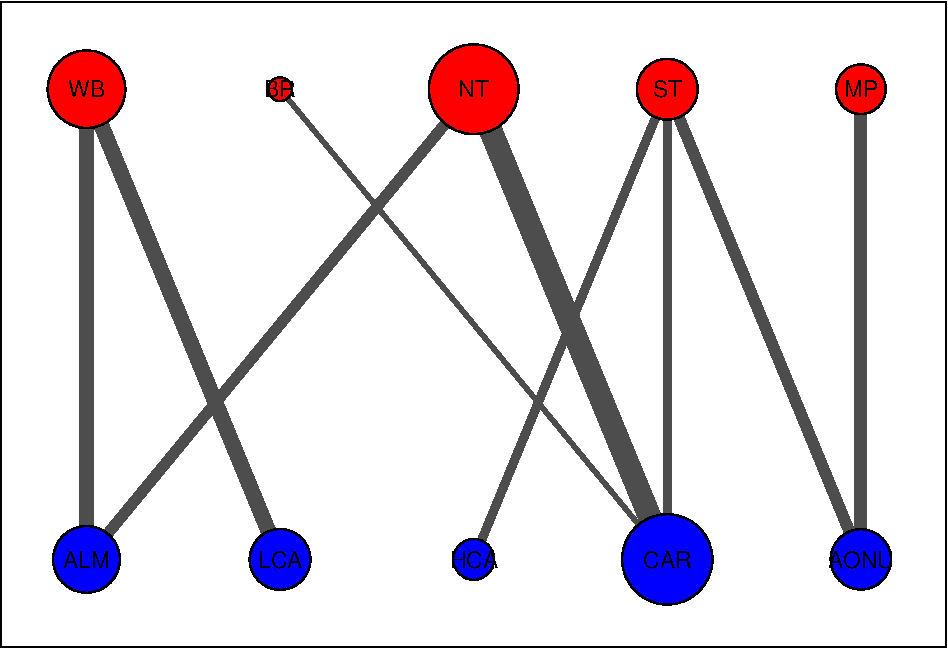
\includegraphics{Mignette_files/figure-latex/unnamed-chunk-5-1.pdf}

In this visualization, node size corresponds to the amount of connectivity with that population and edge size corresponds to the amount of connectivity between the populations. By default, breeding populations are in the top row (red) and nonbreeding/wintering populations are in the bottom row (blue).

This sums up the basics of creating and visualizing a migratory network. We encourage users to explore and build upon the visualization tools we provide (e.g.~overlay the migratory networks on geographic ranges) - the options are endless, enjoy!

\hypertarget{breeding}{%
\chapter{Breeding nodes}\label{breeding}}

Delineating breeding nodes is necessary for our migratory network model for both 1) assignment among populations, and 2) specifying a region for relative abundance. Here, we show how breeding nodes can be delineated by genetically distinct populations on the breeding grounds. In this example, we'll show how to use \href{https://ebird.org/science/status-and-trends}{eBird Status and Trends} data to specify the breeding range and then use genetic data from admixture analyses to specify the spatial extent of the breeding nodes.

\hypertarget{ebirdst}{%
\section{ebirdst}\label{ebirdst}}

In our migratory network analyses, the \href{https://science.ebird.org/en/status-and-trends}{eBird Status and Trends} data is used to delineate the different stages of the annual cycle. Prior to doing anything with eBird Status and Trends data, you will need to download the \texttt{ebirdst} package, and then get access to the data. \textbf{You will need to follow the most up-to-date instructions from the \texttt{ebirdst} developers for getting the abundance data. Currently, that information is here: \url{https://ebird.github.io/ebirdst/}}

To download the package:

\begin{Shaded}
\begin{Highlighting}[]
\CommentTok{\# install.packages("remotes")}
\NormalTok{remotes}\SpecialCharTok{::}\FunctionTok{install\_github}\NormalTok{(}\StringTok{"CornellLabofOrnithology/ebirdst"}\NormalTok{)}
\end{Highlighting}
\end{Shaded}

Then, get access to \texttt{ebirdst} data at \url{https://ebird.org/st/request}. You will receive a key to download \texttt{ebirdst} data and you can enter that key in R:

\begin{Shaded}
\begin{Highlighting}[]
\NormalTok{ebirdst}\SpecialCharTok{::}\FunctionTok{set\_ebirdst\_access\_key}\NormalTok{(}\StringTok{"XXXXX"}\NormalTok{)}
\end{Highlighting}
\end{Shaded}

where \texttt{"XXXXX"} is the key.

By following instructions from the \texttt{ebirdst} developers, you can obtain polygons of the breeding and nonbreeding ranges of avian species (see \url{https://ebird.github.io/ebirdst/} for details).

\hypertarget{creating-the-genoscape}{%
\section{Creating the genoscape}\label{creating-the-genoscape}}

A genoscape is the collection of genetically distinct populations that make up a species' range \citep{ruegg2021american}. Typically, for migratory species, the genoscape describes this population structure on the breeding range because the nonbreeding populations can can contain individuals from different breeding populations.

We will outline the main genoscape creation steps here, but full instructions on creating a genoscape map can be found in Eric Anderson's Github project \href{https://github.com/eriqande/make-a-BGP-map}{Make a Bird Genoscape Project map}. The input data needed for a genoscape are:

\begin{itemize}
\tightlist
\item
  Individual Q-value matrix
\item
  Lat/lon matrix of individuals
\item
  Breeding range polygon
\end{itemize}

The Q-value matrix is obtained from individual admixture analyses (e.g.~Structure, Admixture, \texttt{snmf} fuction from the LEA R-package). Latitude/longitude coordinates are for the individual samples used in the Q-value matrix. Breeding range polygons can be obtained from \texttt{ebirdst} (see previous section).

The \texttt{comyel\_breeding\_data} data set provides admixture results (Q-values) of five genotype clusters for Common Yellowthroat (cite a coye paper) and metadata for the sampled individuals.

\begin{Shaded}
\begin{Highlighting}[]
\NormalTok{Q\_matrix }\OtherTok{\textless{}{-}}\NormalTok{ Mignette}\SpecialCharTok{::}\NormalTok{comyel\_breeding\_data }\SpecialCharTok{\%\textgreater{}\%}
\NormalTok{  dplyr}\SpecialCharTok{::}\FunctionTok{select}\NormalTok{(CA, Midwest, NewEngland, West, Southwest) }\SpecialCharTok{\%\textgreater{}\%}
  \FunctionTok{as.matrix}\NormalTok{()}
\NormalTok{long\_lat\_matrix }\OtherTok{\textless{}{-}}\NormalTok{ Mignette}\SpecialCharTok{::}\NormalTok{comyel\_breeding\_data }\SpecialCharTok{\%\textgreater{}\%}
\NormalTok{  dplyr}\SpecialCharTok{::}\FunctionTok{select}\NormalTok{(Long, Lat) }\SpecialCharTok{\%\textgreater{}\%}
  \FunctionTok{as.matrix}\NormalTok{()}
\NormalTok{cluster\_colors }\OtherTok{\textless{}{-}}  \FunctionTok{c}\NormalTok{(}
  \AttributeTok{CA =} \StringTok{"\#CC0000"}\NormalTok{,}
  \AttributeTok{Midwest =} \StringTok{"\#3399FF"}\NormalTok{,}
  \AttributeTok{NewEngland =} \StringTok{"\#9933CC"}\NormalTok{,}
  \AttributeTok{West =} \StringTok{"\#009933"}\NormalTok{,}
  \AttributeTok{Southwest =} \StringTok{"\#FF6600"}\NormalTok{) }
\end{Highlighting}
\end{Shaded}

We will use a \href{https://github.com/eriqande/TESS3_encho_sen}{modified version} of the \texttt{tess3r} package to create the genoscape rasters.

\begin{Shaded}
\begin{Highlighting}[]
\CommentTok{\# remotes::install\_github("eriqande/TESS3\_encho\_sen")}
\NormalTok{genoscape\_brick }\OtherTok{\textless{}{-}}\NormalTok{ tess3r}\SpecialCharTok{::}\FunctionTok{tess3Q\_map\_rasters}\NormalTok{(}
  \AttributeTok{x =}\NormalTok{ Q\_matrix, }
  \AttributeTok{coord =}\NormalTok{ long\_lat\_matrix,  }
  \AttributeTok{map.polygon =}\NormalTok{ breed\_smooth,}
  \AttributeTok{window =}\NormalTok{ terra}\SpecialCharTok{::}\FunctionTok{ext}\NormalTok{(breed\_smooth)[}\DecValTok{1}\SpecialCharTok{:}\DecValTok{4}\NormalTok{],}
  \AttributeTok{resolution =} \FunctionTok{c}\NormalTok{(}\DecValTok{300}\NormalTok{,}\DecValTok{300}\NormalTok{), }\CommentTok{\# if you want more cells in your raster, set higher}
  \AttributeTok{col.palette =}\NormalTok{ tess3r}\SpecialCharTok{::}\FunctionTok{CreatePalette}\NormalTok{(cluster\_colors, }\FunctionTok{length}\NormalTok{(cluster\_colors)), }
  \AttributeTok{method =} \StringTok{"map.max"}\NormalTok{, }
  \AttributeTok{interpol =}\NormalTok{ tess3r}\SpecialCharTok{::}\FunctionTok{FieldsKrigModel}\NormalTok{(}\DecValTok{10}\NormalTok{),  }
  \AttributeTok{main =} \StringTok{"Ancestry coefficients"}\NormalTok{,}
  \AttributeTok{xlab =} \StringTok{"Longitude"}\NormalTok{, }
  \AttributeTok{ylab =} \StringTok{"Latitude"}\NormalTok{, }
  \AttributeTok{cex =}\NormalTok{ .}\DecValTok{4}
\NormalTok{)}
\FunctionTok{names}\NormalTok{(genoscape\_brick) }\OtherTok{\textless{}{-}} \FunctionTok{colnames}\NormalTok{(Q\_matrix)}

\NormalTok{out.files }\OtherTok{\textless{}{-}} \FunctionTok{paste0}\NormalTok{(}\StringTok{"./comyel/genoscape/comyel\_genoscape\_cluster\_"}\NormalTok{, }\FunctionTok{names}\NormalTok{(genoscape\_brick), }\StringTok{".tif"}\NormalTok{)}
\NormalTok{terra}\SpecialCharTok{::}\FunctionTok{writeRaster}\NormalTok{(terra}\SpecialCharTok{::}\FunctionTok{rast}\NormalTok{(genoscape\_brick), }\AttributeTok{filename =}\NormalTok{ out.files)}
\end{Highlighting}
\end{Shaded}

\textbf{STOP}

The rasters for the genoscape are all that are needed for obtaining information on relative abundance for the different populations. You can continue on to the \protect\hyperlink{abundance}{relative abundance section} if you are ready to do that with the genoscape. Or if you still need to create the wintering nodes, check out the \protect\hyperlink{wintering}{wintering nodes section}. The following section is not necessary for the migratory network but details how to covert genoscape rasters to polygons if the \texttt{mignette} user is interested in doing so.

\hypertarget{genoscape-polygons}{%
\subsection{Genoscape polygons}\label{genoscape-polygons}}

Using the genoscape rasters we will convert them to polygons, using the handy \texttt{scape\_to\_shape()} function. The \texttt{prob\_threshold} parameter specifies the value to determine if a raster cell is included in the polygon for that genoscape. This value should be customized for different species to check for overlap of genoscape polygons, which is not desirable. Setting too high of a threshold will create very small breeding nodes, while too low of a threshold will result in large, overlapping breeding nodes.

\begin{Shaded}
\begin{Highlighting}[]
\NormalTok{genoscape\_files }\OtherTok{\textless{}{-}} \FunctionTok{list.files}\NormalTok{(}\StringTok{"./comyel/genoscape"}\NormalTok{, }
                                     \AttributeTok{full.names =}\NormalTok{ T,}
                                     \AttributeTok{pattern =} \StringTok{"*.tif"}\NormalTok{)}

\NormalTok{genoscape\_raster\_stack }\OtherTok{\textless{}{-}}\NormalTok{ terra}\SpecialCharTok{::}\FunctionTok{rast}\NormalTok{(genoscape\_files)}
\NormalTok{genoscape\_polygon\_sf }\OtherTok{\textless{}{-}}\NormalTok{ mignette}\SpecialCharTok{::}\FunctionTok{scape\_to\_shape}\NormalTok{(}\AttributeTok{x =}\NormalTok{ genoscape\_raster\_stack, }\AttributeTok{prob\_threshold =} \FloatTok{0.5}\NormalTok{)}
\end{Highlighting}
\end{Shaded}

Check out the polygons

\begin{Shaded}
\begin{Highlighting}[]
\FunctionTok{ggplot}\NormalTok{() }\SpecialCharTok{+}
  \FunctionTok{geom\_sf}\NormalTok{(}\AttributeTok{data =}\NormalTok{ genoscape\_polygon\_sf,}\AttributeTok{alpha =} \FloatTok{0.75}\NormalTok{, }\FunctionTok{aes}\NormalTok{(}\AttributeTok{fill =}\NormalTok{ Cluster)) }\SpecialCharTok{+}
  \FunctionTok{scale\_fill\_manual}\NormalTok{(}\AttributeTok{values =}\NormalTok{ cluster\_colors)}
\end{Highlighting}
\end{Shaded}

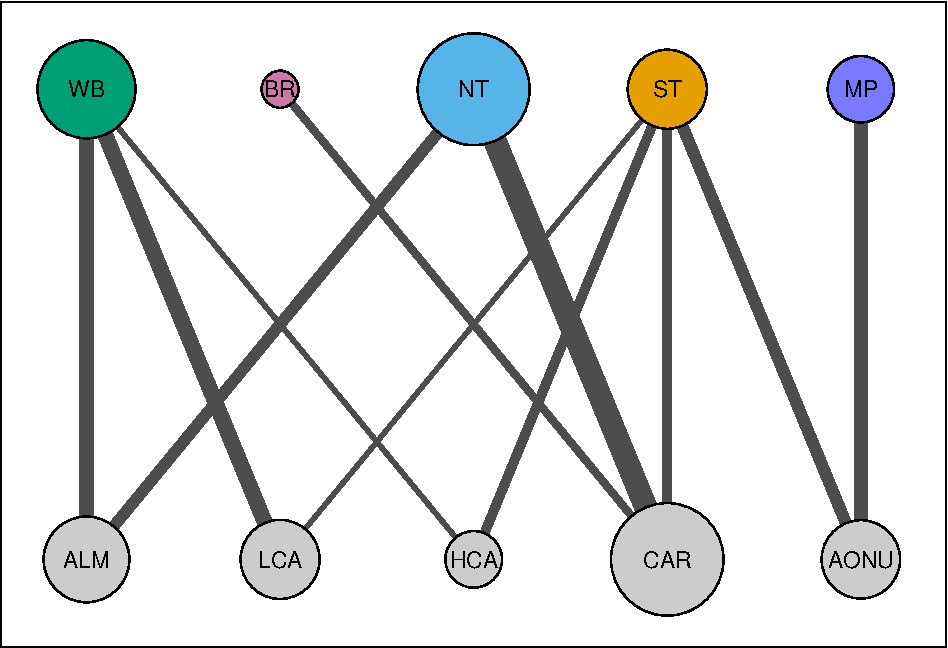
\includegraphics[width=0.7\linewidth]{Mignette_files/figure-latex/unnamed-chunk-7-1}

Check which polygons are overlapping. Each row of the output provides a pair of overlapping polygons (if there are any).

\begin{Shaded}
\begin{Highlighting}[]
\NormalTok{mignette}\SpecialCharTok{::}\FunctionTok{check\_genoscape\_overlap}\NormalTok{(genoscape\_polygon\_sf)}
\end{Highlighting}
\end{Shaded}

\begin{verbatim}
##      [,1]      [,2]        
## [1,] "CA"      "West"      
## [2,] "Midwest" "NewEngland"
## [3,] "Midwest" "West"
\end{verbatim}

Now on to creating the \protect\hyperlink{wintering}{wintering nodes}

\hypertarget{wintering}{%
\chapter{Wintering nodes}\label{wintering}}

For the migratory networks, we will use ecoregions to define the nonbreeding nodes. However, other nonbreeding nodes could be defined by the user instead. If you already have polygons defining your nonbreeding of nodes interest, then continue to the \protect\hyperlink{abundance}{relative abundance section}.

\hypertarget{subsetting-winter-ecoregions}{%
\section{Subsetting winter ecoregions}\label{subsetting-winter-ecoregions}}

The ecoregion data is provided by {[}provide link{]}. The ecoregions are provided in this this package as \texttt{ecoregions\_simple}. We will intersect the ecoregions with the wintering range of the Common Yellowthroat to identify all the ecoregions that overlap with the wintering range.

\begin{Shaded}
\begin{Highlighting}[]
\NormalTok{comyel\_winter }\OtherTok{\textless{}{-}}\NormalTok{ comyel\_range\_smooth }\SpecialCharTok{\%\textgreater{}\%}
\NormalTok{  dplyr}\SpecialCharTok{::}\FunctionTok{filter}\NormalTok{(season }\SpecialCharTok{==} \StringTok{"nonbreeding"}\NormalTok{) }\SpecialCharTok{\%\textgreater{}\%}
\NormalTok{  sf}\SpecialCharTok{::}\FunctionTok{st\_transform}\NormalTok{(}\AttributeTok{crs =} \DecValTok{4326}\NormalTok{) }\SpecialCharTok{\%\textgreater{}\%}
\NormalTok{  sf}\SpecialCharTok{::}\FunctionTok{st\_intersection}\NormalTok{(mignette}\SpecialCharTok{::}\NormalTok{ecoregions\_simple) }\SpecialCharTok{\%\textgreater{}\%}
\NormalTok{  dplyr}\SpecialCharTok{::}\FunctionTok{select}\NormalTok{(Region)}
\end{Highlighting}
\end{Shaded}

\hypertarget{snap-points}{%
\section{Snap points}\label{snap-points}}

Sometimes individuals are not quite within the wintering nodes. Here, we will make sure all sampled individuals get assigned to the nearest ecoregion with the \texttt{mignette} function \texttt{snap\_points()}.

\begin{Shaded}
\begin{Highlighting}[]
\NormalTok{winter.coords }\OtherTok{\textless{}{-}}\NormalTok{ mignette}\SpecialCharTok{::}\NormalTok{comyel\_wintering\_data }\SpecialCharTok{\%\textgreater{}\%}
  \FunctionTok{st\_as\_sf}\NormalTok{(}\AttributeTok{coords=}\FunctionTok{c}\NormalTok{(}\StringTok{"Long"}\NormalTok{,}\StringTok{"Lat"}\NormalTok{)) }\SpecialCharTok{\%\textgreater{}\%}
  \FunctionTok{st\_cast}\NormalTok{(}\StringTok{"MULTIPOINT"}\NormalTok{) }\SpecialCharTok{\%\textgreater{}\%}
  \FunctionTok{st\_set\_crs}\NormalTok{(}\DecValTok{4326}\NormalTok{)}
  
\NormalTok{new.winter.coords }\OtherTok{\textless{}{-}}\NormalTok{ mignette}\SpecialCharTok{::}\FunctionTok{snap\_points}\NormalTok{(winter.coords, comyel\_winter, }\DecValTok{150000}\NormalTok{)}
\end{Highlighting}
\end{Shaded}

\hypertarget{finalize-wintering-nodes}{%
\section{Finalize wintering nodes}\label{finalize-wintering-nodes}}

Now that points have been \emph{snapped} to the appropriate ecoregions, we can further subset all of the ecoregions in which we have actually sampled individuals from. If we haven't sampled individuals from a region, we can't use that region as a node in the migratory connectivity network!

\begin{Shaded}
\begin{Highlighting}[]
\NormalTok{winter\_intersect }\OtherTok{\textless{}{-}} \FunctionTok{st\_intersects}\NormalTok{(comyel\_winter, new.winter.coords, }\AttributeTok{sparse =}\NormalTok{ T)}
\NormalTok{poly\_id }\OtherTok{\textless{}{-}} \FunctionTok{which}\NormalTok{(}\FunctionTok{unlist}\NormalTok{(}\FunctionTok{lapply}\NormalTok{(winter\_intersect, }\ControlFlowTok{function}\NormalTok{(x) }\FunctionTok{length}\NormalTok{(x) }\SpecialCharTok{\textgreater{}} \DecValTok{0}\NormalTok{)))}
\NormalTok{comyel\_winter\_ecoregions }\OtherTok{\textless{}{-}}\NormalTok{ comyel\_winter[poly\_id,]}
\end{Highlighting}
\end{Shaded}

Now on to getting the \protect\hyperlink{abundance}{relative abundance}.

\hypertarget{abundance}{%
\chapter{Relative Abundance}\label{abundance}}

Here, we calculate the relative abundance for the different nodes of the migratory network. The input data for this step are:

\begin{itemize}
\tightlist
\item
  Abundance data (Raster)
\item
  Population ranges (Raster or Vector)
\end{itemize}

Typically, the geographic range of a population will be stored as a vector (e.g., polygon), but in the case of a genoscape, the population ranges can be specified by a raster with q-values. For abundance data, we will use the \href{https://science.ebird.org/en/status-and-trends}{eBird Status and Trends} data, but any abundance data in a raster object can be used.

\hypertarget{get-relative-abundance-for-a-genoscape-raster}{%
\section{Get relative abundance for a genoscape (raster)}\label{get-relative-abundance-for-a-genoscape-raster}}

In the case of a \emph{genoscape} raster with q-values, we will convert the q-values to probabilities of a pixel belonging to that population which is used to weight the abundance values. This is done with a single function \texttt{get\_genoscape\_abunds()}, and outputs a two-column matrix with the population names and the relative abundance of each population.

\begin{Shaded}
\begin{Highlighting}[]
\NormalTok{genoscape\_abunds }\OtherTok{\textless{}{-}} \FunctionTok{get\_genoscape\_abunds}\NormalTok{(}\AttributeTok{genoscape =}\NormalTok{ genoscape, }\AttributeTok{abunds =}\NormalTok{ abunds)}
\end{Highlighting}
\end{Shaded}

\hypertarget{get-relative-abundance-for-a-vector}{%
\section{Get relative abundance for a vector}\label{get-relative-abundance-for-a-vector}}

In the case of vector file delineating populations, we sum abundance across the range of each population. This is done with a single function \texttt{get\_genoscape\_abunds()}, and outputs a two-column matrix with the population names and the relative abundance of each population.

\begin{Shaded}
\begin{Highlighting}[]
\NormalTok{winter\_abunds }\OtherTok{\textless{}{-}} \FunctionTok{get\_vector\_abunds}\NormalTok{(}\AttributeTok{populations =}\NormalTok{ winter\_regions, }\AttributeTok{abunds =}\NormalTok{ abunds)}
\end{Highlighting}
\end{Shaded}

\hypertarget{connectivity}{%
\chapter{Migratory Network Model}\label{connectivity}}

\hypertarget{input-data}{%
\section{Input data}\label{input-data}}

The input data we need for the migratory network model are:

\begin{itemize}
\tightlist
\item
  Relative abundance matrix for each node
\item
  Assignment matrix of individuals among nodes
\end{itemize}

We demonstrate in the previous \protect\hyperlink{abundance}{relative abundance section} how to obtain the relative abundance data needed for the model. The relative abundance data need to be in the following format, with population IDs (same names as in the \emph{assignment} file) in the first column and relative abundance values in the second column. Column names can follow any naming convention when inputting these data into \texttt{mignette}.

\begin{tabular}{l|r}
\hline
Population & Relative\_abundance\\
\hline
ST & 9874.3106\\
\hline
NT & 75628.5485\\
\hline
WB & 27340.7038\\
\hline
AONU & 942.6022\\
\hline
ALM & 1667.3713\\
\hline
CAR & 4850.6727\\
\hline
\end{tabular}

For the assignment matrix, the input data needs to correspond to the following format:

\begin{tabular}{l|r|r|r}
\hline
Breeding & CAR & AONU & ALM\\
\hline
NT & 54 & 0 & 3\\
\hline
ST & 12 & 12 & 0\\
\hline
WB & 1 & 0 & 20\\
\hline
\end{tabular}

where the first column specifies breeding population IDs while subsequent columns are the nonbreeding populations. The values are the number of individuals that connect each node. Depending on the type of assignment data the \texttt{mignette} user has, individual data points may need to be associated with a specific population. For these types of basic spatial analyses, \texttt{mignette} users can check out the \texttt{sf} package, specifically the \texttt{st\_intersection()} function, or whatever geospatial tools they prefer to create these data. Once you have connectivity data in the above format, you can continue with the following sections.

For the following functions, we specify the order of the populations we are using for the model. Here, we are just ordering populations geographically by longitude to facilitate straightforward interpretation of the output.

\begin{Shaded}
\begin{Highlighting}[]
\NormalTok{bnode\_names }\OtherTok{\textless{}{-}} \FunctionTok{c}\NormalTok{(}\StringTok{"WB"}\NormalTok{, }\StringTok{"NT"}\NormalTok{, }\StringTok{"ST"}\NormalTok{)}
\NormalTok{wnode\_names }\OtherTok{\textless{}{-}} \FunctionTok{c}\NormalTok{(}\StringTok{"ALM"}\NormalTok{, }\StringTok{"CAR"}\NormalTok{, }\StringTok{"AONU"}\NormalTok{)}
\end{Highlighting}
\end{Shaded}

\hypertarget{migratory-network-model-jags}{%
\section{Migratory network model (JAGS)}\label{migratory-network-model-jags}}

\hypertarget{preparing-input-data}{%
\subsection{Preparing input data}\label{preparing-input-data}}

The following code provides the necessary data to run the JAGS model. To create the migratory network, the user first creates a text file specifying the JAGS model to be used, providing the name of the file to be saved (\texttt{base\_filename}) and the type of model type (\texttt{model\_type}). Currently \texttt{mignette} supports two model types based on the type of data used to determine assignment of individuals: \texttt{1} indicates that only genetic data were used for assignment, and \texttt{2} indicates that there's assignment data from both genetic and geolocator data. Here, the example only uses genetic data. \texttt{get\_jags\_model()} saves a \texttt{.txt} file with the \texttt{base\_filename} and stores that name as a variable for use in JAGS. We also specify the desired order of the breeding populations (\texttt{bnode\_names}) and the nonbreeding populations (\texttt{wnode\_names}). Finally, we use these as input into the function \texttt{get\_jags\_data()} to prepare the data appropriately for the model.

\begin{Shaded}
\begin{Highlighting}[]
\NormalTok{base\_filename }\OtherTok{\textless{}{-}}\NormalTok{ mignette}\SpecialCharTok{::}\FunctionTok{get\_jags\_model}\NormalTok{(}\AttributeTok{base\_filename =} \StringTok{"amre.genetic.model"}\NormalTok{, }\AttributeTok{model\_type =} \DecValTok{1}\NormalTok{)}
\NormalTok{jags\_data }\OtherTok{\textless{}{-}}\NormalTok{ mignette}\SpecialCharTok{::}\FunctionTok{get\_jags\_data}\NormalTok{(}\AttributeTok{abundance =}\NormalTok{ mignette}\SpecialCharTok{::}\NormalTok{amre\_abundance, }
                           \AttributeTok{assignment =}\NormalTok{ mignette}\SpecialCharTok{::}\NormalTok{amre\_assign,}
                           \AttributeTok{bnode\_names =}\NormalTok{ bnode\_names, }
                           \AttributeTok{wnode\_names =}\NormalTok{ wnode\_names)}
\end{Highlighting}
\end{Shaded}

\hypertarget{running-the-model}{%
\subsection{Running the model}\label{running-the-model}}

Now the user can use the output of \texttt{jags\_data} into JAGS to run the actual model:

\begin{Shaded}
\begin{Highlighting}[]
\NormalTok{parameters }\OtherTok{\textless{}{-}} \FunctionTok{c}\NormalTok{(}\StringTok{"conn\_g"}\NormalTok{)}
\NormalTok{ni }\OtherTok{\textless{}{-}} \DecValTok{500000}
\NormalTok{nt }\OtherTok{\textless{}{-}} \DecValTok{4}
\NormalTok{nb }\OtherTok{\textless{}{-}} \DecValTok{100000}
\NormalTok{nc }\OtherTok{\textless{}{-}} \DecValTok{2}
\NormalTok{jags\_out }\OtherTok{\textless{}{-}} \FunctionTok{autojags}\NormalTok{(jags\_data, }\AttributeTok{inits=}\ConstantTok{NULL}\NormalTok{, parameters, }\FunctionTok{paste0}\NormalTok{(base\_filename,}\StringTok{".txt"}\NormalTok{),}
                      \AttributeTok{n.chains =}\NormalTok{ nc, }\AttributeTok{n.thin =}\NormalTok{nt, }\AttributeTok{iter.increment=}\NormalTok{ni,}
                      \AttributeTok{max.iter =}\NormalTok{ ni}\SpecialCharTok{*}\DecValTok{50}\SpecialCharTok{+}\NormalTok{nb, }\AttributeTok{n.burnin =}\NormalTok{ nb,}
                      \AttributeTok{n.adapt=} \ConstantTok{NULL}\NormalTok{, }\AttributeTok{parallel=}\ConstantTok{TRUE}\NormalTok{)}
\NormalTok{amre\_conn }\OtherTok{\textless{}{-}}\NormalTok{ jags\_out}\SpecialCharTok{$}\NormalTok{mean}\SpecialCharTok{$}\NormalTok{conn\_g}
\NormalTok{amre\_conn}
\end{Highlighting}
\end{Shaded}

\begin{tabular}{r|r|r}
\hline
0.2219310 & 0.0087849 & 0.0000857\\
\hline
0.0557115 & 0.5343810 & 0.0001573\\
\hline
0.0000205 & 0.0538838 & 0.1250444\\
\hline
\end{tabular}

The connectivity between the nodes is provided by the \texttt{conn\_g} parameter of the model, which is accessed from the above code. The rows are the breeding nodes and the columns are the nonbreeding nodes, which we can make more apparent:

\begin{Shaded}
\begin{Highlighting}[]
\FunctionTok{colnames}\NormalTok{(amre\_conn) }\OtherTok{\textless{}{-}}\NormalTok{ wnode\_names}
\FunctionTok{rownames}\NormalTok{(amre\_conn) }\OtherTok{\textless{}{-}}\NormalTok{ bnode\_names}
\NormalTok{amre\_conn}
\end{Highlighting}
\end{Shaded}

\begin{verbatim}
##             ALM         CAR         AONU
## WB 2.219310e-01 0.008784863 8.568762e-05
## NT 5.571149e-02 0.534380974 1.573024e-04
## ST 2.046623e-05 0.053883752 1.250444e-01
\end{verbatim}

\begin{tabular}{l|r|r|r}
\hline
  & ALM & CAR & AONU\\
\hline
WB & 0.2219310 & 0.0087849 & 0.0000857\\
\hline
NT & 0.0557115 & 0.5343810 & 0.0001573\\
\hline
ST & 0.0000205 & 0.0538838 & 0.1250444\\
\hline
\end{tabular}

Voila. A migratory network model is completed. Now, onto \protect\hyperlink{visualization}{visualization}

\hypertarget{visualization}{%
\chapter{Network visualization}\label{visualization}}

We provide functions for basic visualization of the network (\texttt{net\_create()} and \texttt{net\_draw()}). A threshold can be set to remove very weak connectivity for better visualizing the network as shown below.

\begin{Shaded}
\begin{Highlighting}[]
\NormalTok{bnode\_names }\OtherTok{\textless{}{-}} \FunctionTok{c}\NormalTok{(}\StringTok{"WB"}\NormalTok{, }\StringTok{"NT"}\NormalTok{, }\StringTok{"ST"}\NormalTok{)}
\NormalTok{wnode\_names }\OtherTok{\textless{}{-}} \FunctionTok{c}\NormalTok{(}\StringTok{"ALM"}\NormalTok{, }\StringTok{"CAR"}\NormalTok{, }\StringTok{"AONU"}\NormalTok{)}
\CommentTok{\# set threshold for not visualizing minimal connectivity}
\NormalTok{amre\_conn\_test }\OtherTok{\textless{}{-}}\NormalTok{ mignette}\SpecialCharTok{::}\NormalTok{amre\_conn}
\NormalTok{amre\_conn\_test[amre\_conn\_test }\SpecialCharTok{\textless{}} \FloatTok{0.01}\NormalTok{] }\OtherTok{\textless{}{-}} \DecValTok{0}
\NormalTok{net }\OtherTok{\textless{}{-}}\NormalTok{ mignette}\SpecialCharTok{::}\FunctionTok{net\_create}\NormalTok{(amre\_conn\_test, }
                            \AttributeTok{node.names =} \FunctionTok{list}\NormalTok{(bnode\_names, wnode\_names))}
\CommentTok{\#set the display size range for nodes (min and max), default 1{-}10}
\NormalTok{net}\SpecialCharTok{$}\NormalTok{display\_par}\SpecialCharTok{$}\NormalTok{node\_size\_scale}\OtherTok{\textless{}{-}}\FunctionTok{c}\NormalTok{(}\DecValTok{5}\NormalTok{,}\DecValTok{20}\NormalTok{)}
\CommentTok{\#set the display size range for edges (min and max), default 1{-}10}
\NormalTok{net}\SpecialCharTok{$}\NormalTok{display\_par}\SpecialCharTok{$}\NormalTok{edge\_size\_scale}\OtherTok{\textless{}{-}}\FunctionTok{c}\NormalTok{(}\DecValTok{1}\NormalTok{,}\DecValTok{5}\NormalTok{)}
\FunctionTok{plot}\NormalTok{(mignette}\SpecialCharTok{::}\FunctionTok{net\_draw}\NormalTok{(net))}
\end{Highlighting}
\end{Shaded}

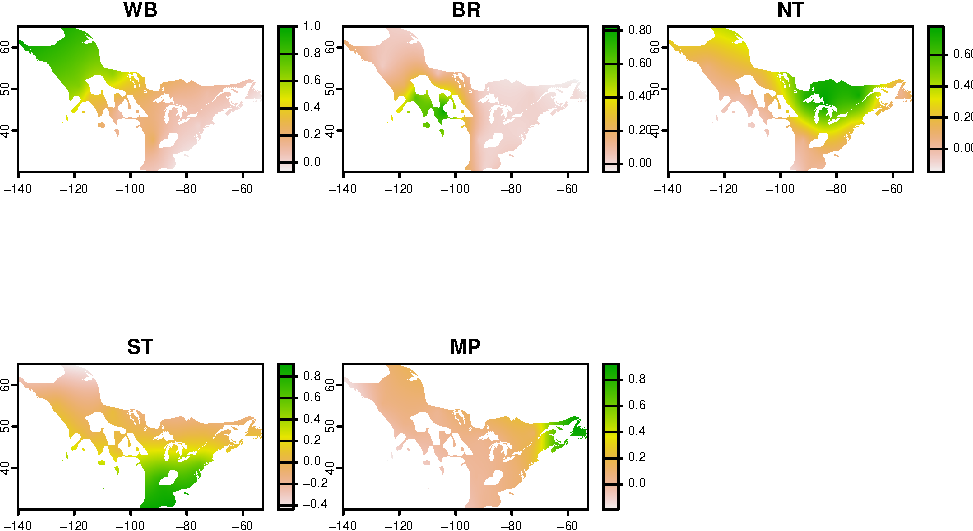
\includegraphics{Mignette_files/figure-latex/unnamed-chunk-15-1.pdf}

In this visualization, node size corresponds to the amount of connectivity with that population and edge size corresponds to the amount of connectivity between the populations. By default, breeding populations are in the top row (red) and nonbreeding/wintering populations are in the bottom row (blue).

This sums up the basics of creating and visualizing a migratory network. We encourage users to explore and build upon the visualization tools we provide (e.g.~overlay the migratory networks on geographic ranges) - the options are endless, enjoy!

  \bibliography{book.bib,packages.bib}

\end{document}
